\documentclass[conference]{IEEEtran}
\IEEEoverridecommandlockouts
% The preceding line is only needed to identify funding in the first footnote. If that is unneeded, please comment it out.
\usepackage{cite}
\usepackage{amsmath,amssymb,amsfonts}
\usepackage{algorithmic}
\usepackage{graphicx}
\usepackage{textcomp}
\usepackage{xcolor}
\usepackage[pdftex]{graphicx}
\usepackage{algorithm}
\usepackage{algpseudocode}

%修改关键字
\renewcommand{\algorithmicrequire}{ \textbf{Input:}}
%UseInput in the format of Algorithm
\renewcommand{\algorithmicensure}{ \textbf{Output:}}
%UseOutput in the format of Algorithm

\def\BibTeX{{\rm B\kern-.05em{\sc i\kern-.025em b}\kern-.08em
    T\kern-.1667em\lower.7ex\hbox{E}\kern-.125emX}}
\begin{document}




\cite{edge-computing}

\begin{table}
\centering
\caption{test table}
\begin{tabular}{|p{3cm}|l|l|r}
\hline
name & class & id & work\\
\hline
Chenxuyang & 1 & 214712244 & student\\
\hline
\end{tabular}
\end{table}



\begin{figure}
\centering
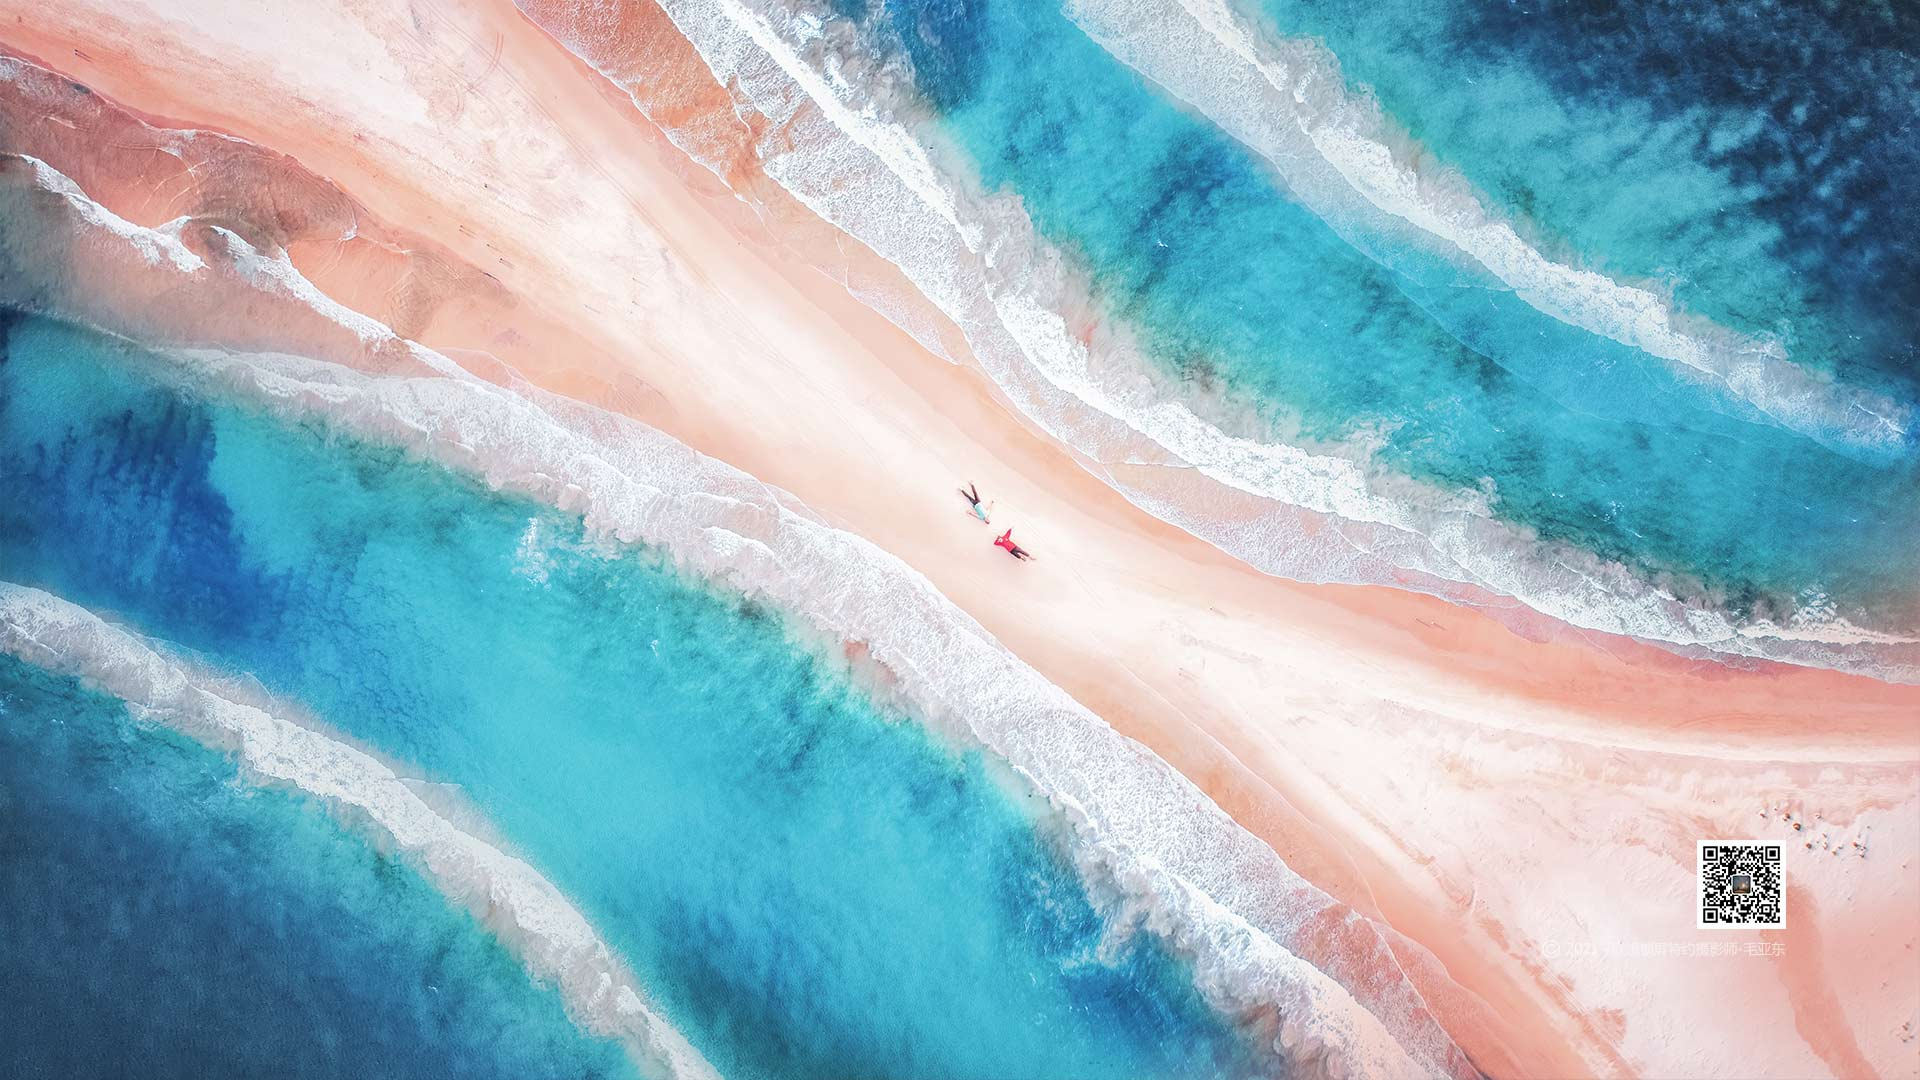
\includegraphics[width=\columnwidth]{1.JPG}

\caption{test figure}
\lable{fig:test-figure}
\end{figure}
hello world,this is first use of the figure~\ref{test-figure}


\begin{algorithm}
\caption{test-algorithm}
\begin{algorithmic}
\State initialize parameters
\For {every epoch}:
\State Do process a.
\If{ a=3 }
 \State Do  copy a to b.
\ElsIf{ a=5 }

\end{algorithmic}
\end{algorithm}


\begin{thebibliography}{00}
\bibitem{b1} G. Eason, B. Noble, and I. N. Sneddon, ``On certain integrals of Lipschitz-Hankel type involving products of Bessel functions,'' Phil. Trans. Roy. Soc. London, vol. A247, pp. 529--551, April 1955.
\bibitem{b2} J. Clerk Maxwell, A Treatise on Electricity and Magnetism, 3rd ed., vol. 2. Oxford: Clarendon, 1892, pp.68--73.
\bibitem{b3} I. S. Jacobs and C. P. Bean, ``Fine particles, thin films and exchange anisotropy,'' in Magnetism, vol. III, G. T. Rado and H. Suhl, Eds. New York: Academic, 1963, pp. 271--350.
\bibitem{b4} K. Elissa, ``Title of paper if known,'' unpublished.
\bibitem{b5} R. Nicole, ``Title of paper with only first word capitalized,'' J. Name Stand. Abbrev., in press.


\end{document}



